\documentclass[a4paper,12pt,obeyspaces,spaces,hyphens]{article}

\def \trainingtitle{Formation développemment Linux embarqué avec Buildroot}
\def \trainingduration{Formation sur site, 3 jours}
\def \agendalanguage{french}
\def \training{buildroot}

\usepackage{agenda}

\begin{document}

\feshowtitle

\feagendasummaryitem{Titre}{
  {\bf \trainingtitle{}}
}
\feagendasummaryitem{Objectifs\newline opérationnels}{
  \begin{itemize}
  \item Être capable de comprendre le principe d'un build system Linux
    embarqué, et comparer Buildroot aux autres outils offrant des
    fonctionnalités similaires.
  \item Être capable de créer un système Linux embarqué simple avec
    Buildroot: créer une configuration, lancer la compilation,
    installer le résultat sur une plateforme embarquée.
  \item Être capable d'ajuster la configuration de Buildroot pour
    construire un système Linux embarqué adapté à des besoins
    spécifiques: choix de la chaîne de compilation croisée, gestion de
    la configuration du noyau Linux, personnalisation du système de
    fichiers racine.
  \item Être capable de créer de nouveaux paquets dans Buildroot pour
    intégrer des applications et bibliothèques supplémentaires dans le
    système Linux embarqué.
  \item Être capable d'utiliser les outils proposés par Buildroot pour
    gérer et analyser le build: suivi des vulnérabilités, comformité
    aux licences open-source, etc.
  \item Être capable de développer et débugger des applications
    user-space Linux dans un contexte où Buildroot est utilisé.
  \item Être capable d'interagir avec la communauté open-source du
    projet Buildroot et de comprendre le fonctionnement interne de
    Buildroot.
  \end{itemize}
}
\feagendasummaryitem{Supports}{
  Vérifiez que le contenu de la formation correspond à vos besoins :
  \newline \url{https://bootlin.com/doc/training/buildroot}.
}
\feagendasummaryitem{Durée}{
  {\bf Trois} jours - 24 h (8 h par jour)
  \newline 40\% de présentations et 60\% de travaux pratiques.
}
\feagendasummaryitem{Formateur}{
  {\bf Thomas Petazzoni}. Thomas est un des quatre
  co-mainteneurs du projet Buildroot. Il participe au projet depuis
  2009, et y a contribué près de 5000 patches.
}
\feagendasummaryitem{Langue}{
  Présentations : Français
  \newline Supports : Anglais
}
\feagendasummaryitem{Public ciblé}{
  Sociétés qui utilisent déjà Buildroot ou qui
  sont intéressées par l'utiliser pour construire leurs systèmes Linux
  embarqué.
}
\feagendasummaryitem{Pré-requis}{
  \begin{itemize}
  \item {\bf Connaissance et pratique des commandes UNIX ou
      GNU/Linux}: les participants doivent être à l'aise avec
    l'utilisation de la ligne de commande Linux. Les participants
    manquant d'expérience sur ce sujet doivent se former par
    eux-mêmes, par exemple en utilisant nos supports de formation
    disponible à l'adresse
    \url{https://bootlin.com/blog/command-line/}.
  \item {\bf Expérience minimale en développement Linux embarqué}: les
    participants doivent avoir une compréhension minimale de
    l'architecture d'un système Linux embarqué: rôle du noyau Linux
    par rapport à l'espace utilisateur, développement d'applications
    espace utilisateur en C. Suivre la formation {\em Linux embarqué}
    de Bootlin, disponible sur
    \url{https://bootlin.com/fr/formation/linux-embarque/} permet de
    remplir ce pré-requis.
  \item {\bf Niveau minimal requis en anglais: B1}, d'après le {\em
      Common European Framework of References for Languages}, pour nos
    sessions animées en anglais.
  \end{itemize}
}
\ferequiredequipmentonsite{}
\feagendasummaryitem{Supports}{
  Copie électronique des présentations et travaux pratiques.
  \newline Version électronique des données pour les travaux
  pratiques..
}

\feagendatwocolumn
{Plateforme matérielle pour les travaux pratiques, option \#1}
{
  Carte {\bf BeagleBone Black}
  \begin{itemize}
  \item Processeur ARM AM335x (single Cortex-A8) de Texas Instruments
  \item Alimentation par USB
  \item 512 MB de RAM
  \item 2 ou 4 GB de stockage eMMC
  \item USB hôte et périphérique
  \item 1 slot Micro SD
  \item Sortie HDMI
  \item Connecteur 2 x 46 broches, pour accéder aux UARTs, bus SPIs, I2Cs, etc.
  \end{itemize}
}
{}
{
  \begin{center}
    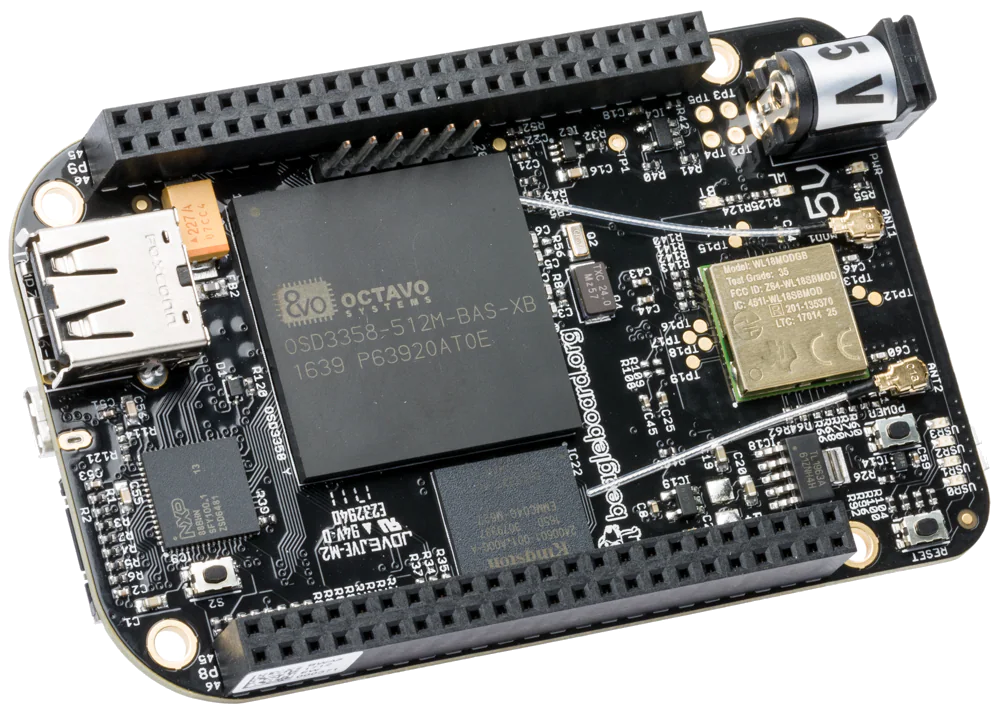
\includegraphics[width=5cm]{../slides/beagleboneblack-board/beagleboneblack.png}
  \end{center}
}

\feagendatwocolumn
{Plateforme matérielle pour les travaux pratiques, option \#2}
{
  Carte {\bf STMicroelectronics STM32MP157D Discovery Kit~1}
  \begin{itemize}
  \item Processeur STM32MP157D (dual Cortex-A7) de STMicroelectronics
  \item Alimentation par USB
  \item 512 MB DDR3L RAM
  \item Ethernet Gigabit
  \item 4 ports USB 2.0 hôte
  \item 1 port USB-C OTG
  \item 1 slot Micro SD
  \item Debugger ST-LINK/V2-1
  \item Connecteurs compatibles Arduino
  \item Codec audio, boutons, LEDs
  \end{itemize}
}
{}
{
  \begin{center}
    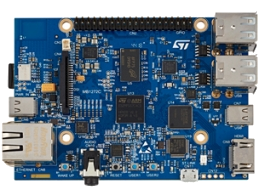
\includegraphics[width=5cm]{../slides/discovery-board-dk1/discovery-board-dk1.png}
  \end{center}
}

\section{1\textsuperscript{er} jour - Matin}

\feagendatwocolumn
{Cours - Introduction à Buildroot et aux systèmes de build}
{
  \begin{itemize}
  \item Architecture générale d'une système Linux embarqué
  \item Choix entre systèmes de build et distributions binaires
  \item Rôle d'un système de build
  \item Comparaison des systèmes de build existants
  \end{itemize}
}
{Cours - Présentation de Buildroot}
{
  \begin{itemize}
  \item Points clés autour du projet
  \item Téléchargement des sources de Buildroot
  \item Configuration simple de Buildroot
  \item Exécution d'une premières compilation
  \end{itemize}
}
\\
\feagendatwocolumn
{TP - Utilisation simple de Buildroot}
{
  \begin{itemize}
  \item Téléchargement et configuration de Buildroot
  \item Configurer et compiler un système simple avec Buildroot, pour la
        carte BeagleBone Black
  \item Flasher et tester le système générer sur la carte BeagleBone
        Black.
  \end{itemize}
}
{Cours - Gestion de la compilation et de la configuration}
{
  \begin{itemize}
  \item Compilation en dehors des sources
  \item Utiliser et créer des fichiers {\em defconfigs}
  \item Fragments de {\em defconfigs}
  \item Autres astuces pour la compilation
  \end{itemize}
}


\section{1\textsuperscript{er} jour - Après-midi}

\feagendatwocolumn
{Cours - Sources de Buildroot et arborescence des fichiers générés}
{
  \begin{itemize}
  \item Détails sur l'organisation du code source de Buildroot
  \item Détails sur l'arborescence des fichiers générés
  \end{itemize}
}
{Cours - Chaînes de compilation {\em toolchains} dans Buildroot}
{
  \begin{itemize}
  \item Les différents possibilités d'usage de chaînes de compilation
	dans Buildroot.
  \item Tour d'horizon des options liées aux chaînes de compilation.
  \item Utilisation de chaînes des compilation binaires, comme
	celles de Bootlin. Détails sur les fonctionnalités
        {\em multilib} et l'intégration des toolchains dans Buildroot.
  \item Génération de toolchains sur mesure avec {\em Crosstool-NG},
	et leur utilisation comme chaînes externes.
  \end{itemize}
}

\feagendatwocolumn
{Cours - Gestion de la configuration du noyau Linux}
{
  \begin{itemize}
  \item Charger, modifier et sauvegarder la configuration du noyau.
  \end{itemize}
}
{Cours - Construction du système de fichier racine dans Buildroot}
{
  \begin{itemize}
  \item Comprendre comment Buildroot construit le système de fichiers
	racine: {\em skeleton}, installation de composants, {\em
        overlays}, scripts {\em post-build} et {\em post-image}.
  \item Personnalisation du contenu du système de fichiers
  \item Configuration du système: sélection de la {\em console},
	plusieurs méthode de gestion de {\tt /dev}, les différentes
	implémentations d'{\tt init}, etc.
  \item Comprendre comment Buildroot génère les images de systèmes de
	fichiers.
  \end{itemize}
}

\feagendaonecolumn
{TP - Personnalisation du système de fichiers}
{
  \begin{itemize}
  \item Exploration des fichiers générés
  \item Personnalisation du système de fichiers racine en utilisant un {\em rootfs overlay}
  \item Personnaliser le noyau avec des correctifs et des options de
	configuration supplémentaires
  \item Rajout de nouveaux composants
  \item Utilisation de fichiers {\em defconfig} et compilation en
	dehors des sources.
  \end{itemize}
}

\section{2\textsuperscript{ème} jour - Matin}

\feagendatwocolumn
{Cours - Infrastructure de téléchargement dans Buildroot}
{
  \begin{itemize}
  \item Méthodologie de téléchargement
  \item Site primaire et sites de backup, compilation en mode déconnecté
  \item Téléchargement via systèmes de contrôle de versions,
	vérification d'intégrité
  \item Cibles {\em make} en rapport avec les téléchargements
  \end{itemize}
}
{Cours - Introduction à GNU Make}
{
  \begin{itemize}
  \item Éléments de base des règles de make
  \item Définition et utilisation de variables
  \item Conditions et fonctions
  \item Écriture de recettes
  \end{itemize}
}

\feagendatwocolumn
{Cours - Intégration de nouveaux composants dans Buildroot}
{
  \begin{itemize}
  \item Comment rajouter de nouveaux paquetages au système de
	configuration de Buildroot
  \item Comprendre les différentes infrastructures de paquetages : pour
	des composants {\em generic}, {\em autotools}, {\em CMake}, {\em
	Python} et autres
  \item Écriture un fichier \code{Config.in} pour un composant: comment
    exprimer des dépendances vers d'autres composants, vers des options
    de toolchains, etc.
  \item Détails sur l'écriture d'une recette pour un composant :
	description de l'emplacement du code source, de la méthode de
	téléchargement, de configuration, de compilation et
	d'installation, gestion des dépendances, etc. 
  \end{itemize}
}
{TP - Nouveaux composants dans Buildroot}
{
  \begin{itemize}
  \item Création d'un nouveau paquetage pour {\em nInvaders}
  \item Comprendre comment rajouter des dépendances
  \item Ajouter des correctifs pour {\em nInvaders} pour prendre en
	charge le contrôle via un {\em Nunchuk}
  \end{itemize}
}

\section{2\textsuperscript{ème} jour - Après-midi}

\feagendatwocolumn
{Cours - Notions avancées sur les paquetages}
{
  \begin{itemize}
  \item Rapport de licences
  \item Prise en charge des correctifs: ordre d'application et format,
	répertoire global pour les correctifs, etc.
  \item Utilisateur, droit d'accès, tables de fichiers devices
  \item Script d'init et fichiers unitaires pour systemd
  \item Scripts de configuration
  \item Compréhension des {\em hooks}
  \item Surcharger des commandes
  \item Gestion des paquetages legacy
  \item Paquetages virtuels
  \end{itemize}
}
{TP - Paquetages avancés}
{
  \begin{itemize}
  \item Packager une application avec une dépendance obligatoire et
    une dépendance optionnelle
  \item Packager une bibliothèque, hébergée sur GitHub
  \item Utilisation de {\em hooks} pour ajuster les paquetages
  \item Rajouter un correctif à un paquetage
  \end{itemize}
}

\section{3\textsuperscript{ème} jour - Matin}

\feagendatwocolumn
{Cours - Analyse d'une compilation: licences, dépendances, temps de
construction}
{
  \begin{itemize}
  \item Utilisation de l'infrastructure de gestion des informations
	légales
  \item Représentation graphique des dépendances entre paquetages
  \item Collecte d'informations et représentation du temps de
	compilation
  \end{itemize}
}
{Cours - Sujets avancés}
{
  \begin{itemize}
  \item \code{BR2_EXTERNAL} pour stocker des personnalisations à
	l'extérieur des sources de Buildroot
  \item Cibles make spécifiques pour les paquetages
  \item Comprendre les recompilations
  \item Astuces pour compiler plus vite
  \end{itemize}
}

\feagendaonecolumn
{TP - Sujets avancés}
{
  \begin{itemize}
  \item Utilisation des capacités de génération de graphes de temps de
	compilation
  \item Génération de graphes de dépendances
  \item Utilisation du rapport sur les licences, et ajout d'informations
	légales à vos propres paquetages 
  \item Utilisation de \code{BR2_EXTERNAL}
  \end{itemize}
}

\section{3\textsuperscript{ème} jour - Après-midi}

\feagendatwocolumn
{Cours - Développement applicatif avec Buildroot}
{
  \begin{itemize}
  \item Utilisation de Buildroot pendant le développement d'applications
  \item Utilisation de l'environnement de Buildroot pour compiler des
	applications en dehors de Buildroot
  \item Générer un SDK pour d'autres développeurs
  \item Débug à distance avec Buildroot
  \end{itemize}
}
{TP - Développement applicatif avec Buildroot}
{
  \begin{itemize}
  \item Compiler et exécuter votre propre application
  \item Débug à distance de votre application
  \item Utilisation de \code{<pkg>_OVERRIDE_SRCDIR}
  \end{itemize}
}

\feagendatwocolumn
{Cours - Comprendre les mécanismes internes de Buildroot}
{
  \begin{itemize}
  \item Description détaillée du processus de compilation de Buildroot:
    	toolchain, paquetages, construction du système de fichiers race,
	fichiers {\em stamp}, etc.
  \item Comprendre les paquetages virtuels.
  \end{itemize}
}
{Cours - Obtenir de l'aide et s'impliquer, nouveautés dans Buildroot}
{
  \begin{itemize}
  \item Obtenir de l'assistance technique: {\em Bugzilla}, {\em liste de
	discussion}, {\em IRC}
  \item Contribuer: comprendre le processus de développement, comment
    soumettre des correctifs
  \item Nouveautés dans Buildroot: résumé des principaux changements
    depuis les deux dernières années
  \end{itemize}
}

\end{document}
